\documentclass[conference,a4paper]{IEEEtran}
\usepackage{fontspec}
\IfFontExistsTF{Times New Roman}{\setmainfont{Times New Roman}}{\setmainfont{TeX Gyre Termes}}
\usepackage{amsmath,amssymb,graphicx,booktabs,url}
\usepackage{balance}
\usepackage[hidelinks]{hyperref}
\graphicspath{{../figures/}{figures/}}
\newcommand{\runid}{20260915T050327853533Z-seed42}
\title{Personalized Game Recommendation for Users with Sparse Interaction Histories}
\author{\IEEEauthorblockN{Nguyễn Bá Hùng (523K0006) and Nguyễn Bảo Long (523K0014)}
\IEEEauthorblockA{Faculty of Information Technology, Ton Duc Thang University\\
Data Mining and Knowledge Discovery --- Group 6, Class 23K50201\\
Lecturer: Hoàng Anh}}
\begin{document}
\maketitle
\begin{abstract}
This midterm project investigates game recommendation when a held-out user supplies only one, three, or five positive interactions. A reproducible pipeline combines historical UCSD Steam reviews and metadata, producing a 20,000-user sample with 37,391 cleaned positive pairs. User-disjoint splitting and train-only feature fitting yield a common catalog of 2,235 games. Most Popular, tag/genre TF-IDF, and sparse item-based collaborative filtering are compared using identical candidates and nested support sets with fixed queries. The common development-test cohort contains 123 users; shorter observed histories are evaluated separately. At five support games, Popular reaches Recall@10 of 0.224661 and NDCG@10 of 0.161285, exceeding Content and ItemCF, while personalized methods achieve wider catalog coverage. The report retains these negative personalization results and examines no-hit frequency, target popularity, and measurement limitations. A local inference benchmark and independent artifact audit support reproducibility. The final section describes a full-stack application that serves verified artifacts and model-derived explanations. BPR, hybrids, semantic embeddings and multi-seed extensions belong to the separate final-term version, outside this frozen M0--M3 submission.
\end{abstract}
\begin{IEEEkeywords}
game recommendation, sparse history, TF-IDF, item-based collaborative filtering, leakage prevention
\end{IEEEkeywords}

\section{Introduction}
Recommending games from a small number of declared preferences requires distinguishing missing information from negative preference. A user who supplies one favorite game may have played many others; a user with no positive review in a historical dataset is not necessarily a new player. This project therefore studies \emph{limited available history}, rather than claiming that simulated truncation directly represents inactivity in the real world.

The task is Top-10 ranking over eligible games. A support set contains the interactions that the model may use to form a profile, while a disjoint query contains withheld positive targets. The study asks which of three baselines performs best at support sizes one, three, and five, and how ranking quality relates to catalog exposure and inference cost. A second, separate cohort covers users with short positive histories observed in the source. Zero-support behavior is tested as fallback functionality, not as an offline personalized-ranking experiment.

The midterm contribution is an auditable data-mining pipeline connected to a working product. It includes real-data inspection, deterministic preprocessing, user-disjoint evaluation, train-only feature construction, validation selection, saved predictions, and measured results. No new recommendation algorithm is claimed. The current evidence also does not support a claim that personalization improves accuracy: Popular outperforms the implemented Content and ItemCF baselines.

\section{Data and Exploratory Analysis}
\subsection{Source and positive interactions}
The input combines the UCSD Steam V1 review archive with Steam V2 metadata, joined by application identifier rather than title \cite{ucsd}. Downloaded files contain 6,935,922 and 2,740,516 bytes, respectively; SHA-256 hashes and provenance are recorded in local manifests. The review file stores a user and a list of reviews per line as Python dictionary literals. The parser uses \texttt{ast.literal\_eval}, validates fields, and reports malformed records by line number.

Metadata without identifiers is removed, duplicate metadata identifiers retain the first record, and titles fall back to \texttt{app\_name}. Reviews are flattened and deduplicated by user--item pair. Conflicting labels would exclude a pair; none were observed. Only \texttt{recommend is True} forms a positive label. Raw negative reviews are not relabeled as positive, and unobserved games are not verified negatives. No user k-core filter removes sparse users.

The full survey contains 25,485 unique users and 59,305 reviews. After deduplication there are 51,692 unique positive pairs, of which 4,200 cannot be joined to metadata. The joined data contain 47,492 positive pairs over 2,869 items. Cross-version joining can introduce historical mismatch and selection bias, even with exact identifier matching. Review text, helpful votes, sentiment, titles, and artwork are not model features.

\subsection{Sampling and sparsity}
An initial 5,000-user feasibility sample retained only 14 common validation and 23 common test users after catalog filtering. The project expanded to 20,000 users before examining model quality, preserving the original sample. Sampling retains all cleaned positive interactions of selected users. Table~\ref{tab:data} separates the sampled population from the training catalog and evaluated cohort.

\begin{table}[t]
\caption{Frozen M1 dataset and evaluation scope}\label{tab:data}
\centering\small
\begin{tabular}{lr}\toprule
Quantity & Value\\\midrule
Sample users / positive pairs & 20,000 / 37,391\\
Sample items & 2,614\\
Train / validation / test users & 14,000 / 3,000 / 3,000\\
Training positives / catalog items & 26,174 / 2,235\\
Training matrix sparsity & 99.91635\%\\
Common validation / test users & 125 / 123\\
Short-history test users, $k=1/3$ & 986 / 212\\\bottomrule
\end{tabular}
\end{table}

The sample contains 1,855 users with zero cleaned positives and 10,229 with one (Fig.~\ref{fig:history}). They remain visible in descriptive statistics but cannot supply both a nonempty support and an independent query. The maximum observed history is ten; the project does not infer a behavioral explanation for this bound or claim results for above-20 histories.

\begin{figure}[t]
\centering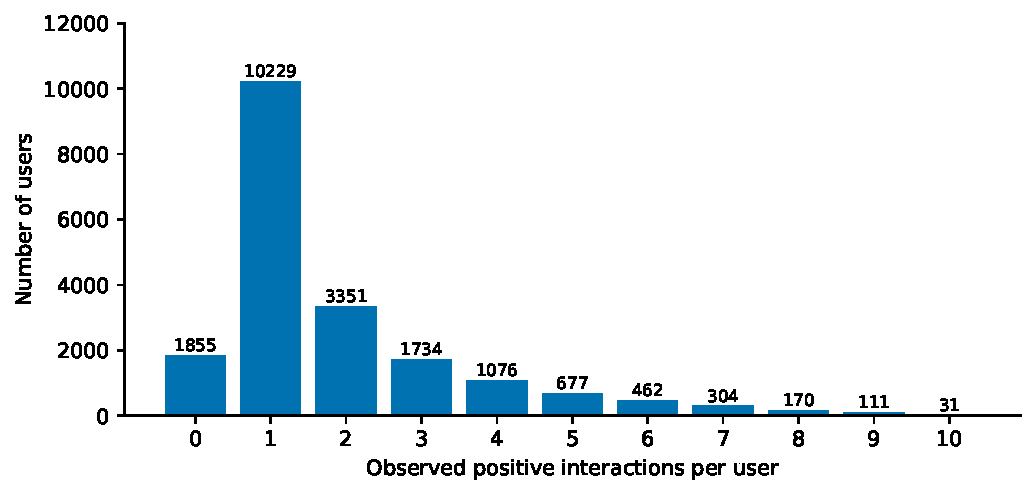
\includegraphics[width=\columnwidth]{history.pdf}
\caption{Observed positive histories in the sampled population. The ranking cohort is much smaller than 20,000 users.}\label{fig:history}
\end{figure}

The \texttt{posted} field is a review date, not game-play time. The source survey parses 49,186 dates with sufficient year information and counts 10,119 incomplete or invalid dates. Missing years are not inferred. Random holdout is consequently used; the experiment is static historical evaluation, not future-behavior forecasting. Review authors and catalog-filtered users are not assumed to represent all Steam players.

\section{Baseline Methods}
\subsection{Common representation and Popular}
Let $R\in\{0,1\}^{|U_{tr}|\times|C|}$ be the training interaction matrix, $C$ the common catalog, $S_u$ a supplied support set, and $Q_u$ the valid query. Each catalog item has at least one training positive and joined metadata. Sparse CSR storage represents the 26,174 observed entries without a dense user--item matrix.

Most Popular uses only training counts:
\begin{equation}
s_{pop}(i)=\sum_{u\in U_{tr}}R_{ui}.
\end{equation}
The recommender excludes support and hidden items, sorts by descending score, and resolves ties through stable lexicographic source identifiers. Increasing support can improve this baseline's metric by removing already-known candidates, even though the model does not learn a personal preference vector.

\subsection{Content TF-IDF and cosine}
Content features are deduplicated, case-folded tags and genres with field prefixes. Multiword labels remain atomic; \texttt{tags:action} and \texttt{genres:action} are distinct. The saved feature matrix contains 349 dimensions. Vocabulary and IDF are fit only on training-catalog metadata. Smoothed TF-IDF follows the library convention \cite{tfidf}:
\begin{equation}
\operatorname{idf}(t)=\log\frac{1+|C|}{1+\operatorname{df}(t)}+1,
\qquad \mathbf{x}_i=\frac{\mathbf{v}_i}{\|\mathbf{v}_i\|_2}.
\end{equation}
Here $v_{it}=\operatorname{tf}_{it}\operatorname{idf}(t)$. Because tokens are sets within an item, presence has term frequency one. The profile and score are
\begin{equation}
\mathbf{p}_u=\frac{\sum_{j\in S_u}\mathbf{x}_j}
{\|\sum_{j\in S_u}\mathbf{x}_j\|_2},
\qquad s_{content}(u,i)=\mathbf{x}_i^T\mathbf{p}_u.
\end{equation}
Normalizing a sum is equivalent to normalizing its mean. Query items never enter the profile. Additional support can rotate the profile away from a target, so accuracy need not increase monotonically. Equal support weighting also compresses multiple interests into one direction; no learned attention, recency weight, or separate interest cluster is implemented.

The score is interpretable through feature products $x_{it}p_{ut}$. These contributions support explanations but do not estimate the probability that a user will like a game. Metadata availability is also not evidence of predictive usefulness: every training item has a nonempty vector, yet broad tags may distinguish preferences poorly.

\subsection{Sparse item-based collaborative filtering}
Item-based CF relates games through shared training users, following the item-neighborhood principle \cite{sarwar}. The project uses binary cosine rather than a rating-centered estimator:
\begin{equation}
\operatorname{sim}(i,j)=\frac{R_{:i}^{T}R_{:j}}
{\|R_{:i}\|_2\|R_{:j}\|_2},\qquad
s_{CF}(u,i)=\sum_{j\in S_u}W_{ji}.
\end{equation}
The implementation computes sparse products in blocks of 128 items, removes self and zero similarities, and retains row-wise Top-$N$ neighbors in $W$. Truncation can make $W$ asymmetric even when the original cosine matrix is symmetric. Scores are unnormalized sums; no shrinkage or candidate-specific denominator is added.

The neighborhood grid is $N\in\{20,50,100\}$. Mean validation common NDCG@10 across the three support levels is 0.041283, 0.053553, and 0.067556, respectively. The selected value is 100, with smaller $N$ as the predefined tie-break. This is the best tested value, not a claim of global optimality. Popular and Content have no tuning grid in this milestone.

\subsection{Fallback and artifacts}
Content and ItemCF use popularity when no known support exists or the entire score vector lacks positive signal. Fallback is decided before candidate exclusion. A partially zero-scored candidate set is not supplemented by a different popularity order; zero-score results can remain according to the stable tie rule and must not receive invented similarity explanations.

The inference function receives support and optional hidden items, but no query. NPZ/JSON artifacts preserve sparse features, interactions, neighborhoods, popularity, IDF, catalog mappings, and schema metadata. Loading disables pickle and checks shape, finite values, schema, and integrity hashes. Model fitting is separated from request-time inference.

\section{Experimental Protocol}
\subsection{User split and nested support}
Users are split 70/15/15 using a stable input order and seed 42. Training, validation, and test users are disjoint. All baselines share the same case manifests, catalog, and exclusion policy. A common-cohort user must have at least six positives. A deterministic permutation, controlled by seed and a hash of the user identifier, allocates the first five items to a support pool and the remainder to a query.

\begin{figure}[t]
\centering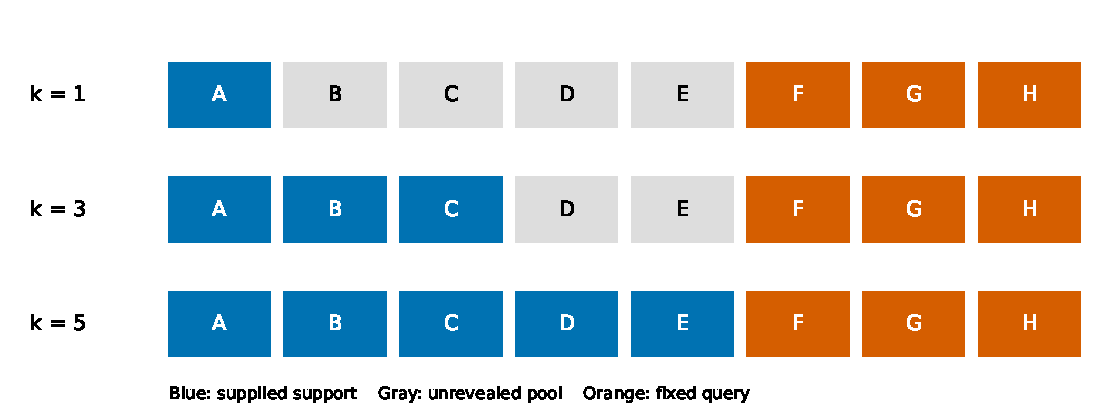
\includegraphics[width=\columnwidth]{protocol.pdf}
\caption{Illustrative nested support. The same query is retained; unrevealed pool items are not reassigned as targets. Letters are hypothetical.}\label{fig:protocol}
\end{figure}

Support sets of size one, three, and five are prefixes of the same pool (Fig.~\ref{fig:protocol}). The query remains fixed. At smaller support sizes, unrevealed pool items can remain candidates but do not count as query hits. Only actually supplied support is excluded. This policy avoids using hidden support information to filter candidates and makes the incomplete-positive nature of evaluation explicit.

Common-cohort admission requires all five pool items in the training catalog and a nonempty filtered query. Of 167 eligible validation users, 40 fail the support check and two more have empty queries. Of 159 eligible test users, 35 fail support and one more has an empty query. The retained counts are 125 and 123. Query audit counts outside the catalog are 11/334 and 10/333 on all eligible validation/test users, including support-rejected users. Filtering is reported because it favors items observed in training.

\subsection{Candidates, cohorts, and selection}
Evaluation uses the full catalog minus supplied support, giving 2,234, 2,232, and 2,230 candidates. It does not sample negative candidates. The short-observed cohort requires between $k+1$ and five positives, producing 986 test users at $k=1$ and 212 at $k=3$. There is no valid $k=5$ short cohort; its metrics are null, not zero. Cross-$k$ changes in that cohort cannot be attributed solely to support length because membership differs.

Validation determines ItemCF's neighborhood setting. Trials and selection are saved before development-test scores are computed. The existing test has been viewed during development and is explicitly not an untouched final test. Zero-support tags are not inferred from query metadata; the application accepts independently declared tags, but corresponding offline quality is unmeasured.

\subsection{Metrics}
Recall@10 is $|L_u^{10}\cap Q_u|/|Q_u|$, where $L_u^{10}$ is the recommendation list. Binary NDCG uses the discounted-gain principle \cite{ndcg}:
\begin{equation}
\operatorname{NDCG@10}(u)=
\frac{\sum_{r=1}^{10}\operatorname{rel}_r/\log_2(r+1)}
{\sum_{r=1}^{\min(10,|Q_u|)}1/\log_2(r+1)}.
\end{equation}
Metrics are computed per user and macro-averaged. Empty queries are counted and excluded before evaluation. For illustration, three targets with hits at ranks one and four yield Recall $2/3$ and NDCG about 0.671386; this is a calculation example, not a dataset result.

Coverage is the fraction of catalog items recommended to at least one user. ILD averages $1-\operatorname{cosine}$ across pairs with nonzero content vectors, excluding and counting lists with fewer than two valid vectors. Mean recommendation popularity uses positive training-user counts. These statistics describe exposure and metadata distance; they do not directly measure satisfaction or fairness. Popularity-bias research motivates examining exposure alongside relevance \cite{bias}.

\section{Results and Discussion}
\subsection{Common-cohort quality}
Table~\ref{tab:quality} uses the frozen run \texttt{\runid}. Popular leads all support levels. At $k=5$, its Recall is 0.224661 versus 0.064905 for Content and 0.122358 for ItemCF. NDCG follows the same ordering. No result is replaced because a personalized model underperforms.

\begin{table}[t]
\caption{Common development-test cohort, 123 users}\label{tab:quality}
\centering\small
\begin{tabular}{lrrrr}\toprule
Model & $k$ & Recall@10 & NDCG@10 & Coverage\\\midrule
Popular & 1 & .215176 & .146111 & .004922\\
Content & 1 & .038889 & .034630 & .255481\\
ItemCF & 1 & .036450 & .023343 & .285906\\
Popular & 3 & .220596 & .156797 & .005817\\
Content & 3 & .046341 & .024265 & .219687\\
ItemCF & 3 & .089566 & .054812 & .302013\\
Popular & 5 & .224661 & .161285 & .006711\\
Content & 5 & .064905 & .042373 & .187919\\
ItemCF & 5 & .122358 & .084229 & .283221\\\bottomrule
\end{tabular}
\end{table}

\begin{figure}[t]
\centering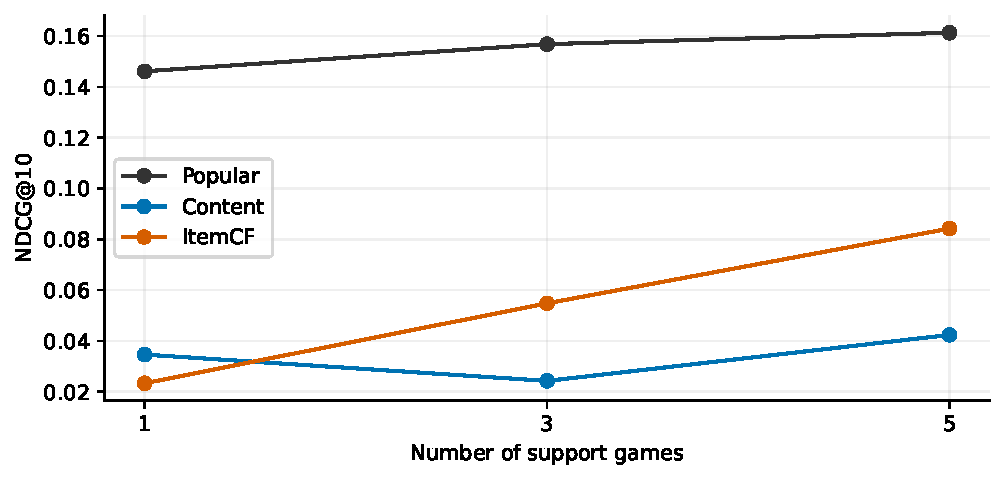
\includegraphics[width=\columnwidth]{ndcg.pdf}
\caption{NDCG@10 on the same held-out users and fixed queries. Content is nonmonotonic as support increases.}\label{fig:ndcg}
\end{figure}

ItemCF improves as support grows in this common cohort. Content's NDCG instead declines at $k=3$ before recovering at $k=5$ (Fig.~\ref{fig:ndcg}). Additional metadata can change the profile direction rather than simply add useful evidence. These are observations from one seed, not causal demonstrations or statistical guarantees. Popular's smaller improvement can also reflect removal of more known items from candidates.

The exposure trade-off is substantial. At $k=5$, Popular covers about 0.67\% of the catalog, Content 18.79\%, and ItemCF 28.32\%. Their ILD values are 0.737230, 0.538722, and 0.865081; average training popularity is 719.221, 36.271, and 240.493. Content can cover many items across users while generating relatively homogeneous lists within each user. Wider coverage therefore does not imply either higher relevance or higher within-list diversity.

\begin{figure}[t]
\centering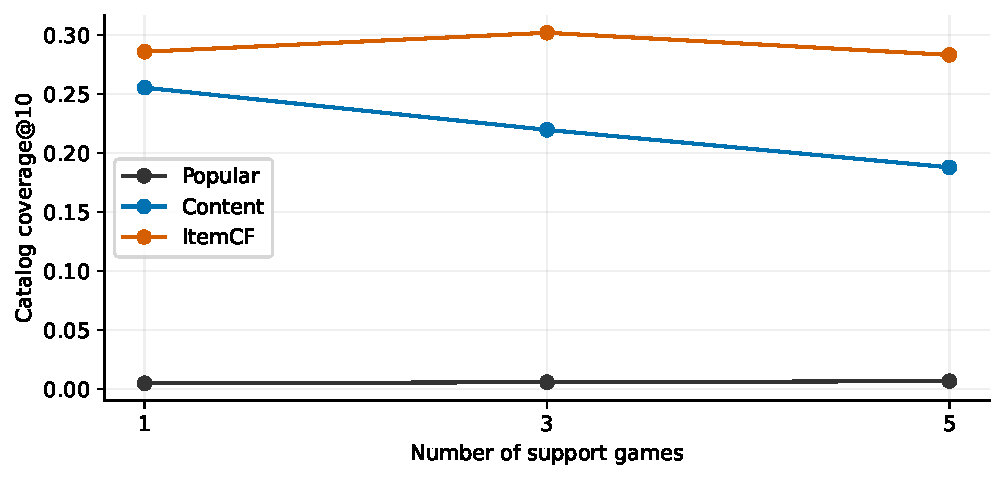
\includegraphics[width=\columnwidth]{coverage.pdf}
\caption{Catalog exposure across support sizes. Broader coverage does not imply stronger target recovery.}\label{fig:coverage}
\end{figure}

This distinction is important for interpreting a practical discovery interface. A system optimized only for the current query metric may repeatedly expose the popular head. A system that increases exposure without recovering relevant targets may offer variety without usefulness. The present experiment establishes neither that one objective should replace the other nor that a particular weighting is optimal. It instead supplies a baseline against which a validation-selected hybrid or reranker can be evaluated.

The representation also constrains interpretation of diversity. ILD uses the same tags and genres as Content, so a list of games with different labels is diverse by that definition even when users might perceive them as similar in difficulty or visual style. Conversely, games with shared genre labels can provide very different experiences. Future user-facing claims about discovery should therefore separate measurable catalog statistics from unmeasured perceptions.

\subsection{Short histories and failure analysis}
Table~\ref{tab:short} reports short-observed histories separately. Popular also leads these comparisons. Different user populations at $k=1$ and $k=3$ prevent interpreting their average differences as a controlled support-size effect. Observed record length does not establish real-world activity level.

\begin{table}[t]
\caption{Short-observed development-test cohorts}\label{tab:short}
\centering\small
\begin{tabular}{lrrrr}\toprule
Model & $k$ & Users & Recall@10 & NDCG@10\\\midrule
Popular & 1 & 986 & .322262 & .212619\\
Content & 1 & 986 & .045892 & .034621\\
ItemCF & 1 & 986 & .108942 & .068714\\
Popular & 3 & 212 & .283019 & .186630\\
Content & 3 & 212 & .084906 & .044075\\
ItemCF & 3 & 212 & .143868 & .081467\\\bottomrule
\end{tabular}
\end{table}

At common-cohort $k=5$, the no-hit counts are 72/123 for Popular, 109/123 for Content, and 95/123 for ItemCF. Even the strongest baseline misses every known query target for many users. Conversely, no hit does not imply that all recommendations are disliked, because query labels cover only a subset of possible interests. No fallback occurs in these three common-test runs.

A deterministic descriptive case selects the first sorted internal user key for which Popular has a hit and both personalized models have none. Support includes Surgeon Simulator, Prison Architect, Left 4 Dead 2, Dota 2, and Counter-Strike: Global Offensive; query contains Terraria, Half-Life 2, and Cities: Skylines. Popular places Terraria fifth, obtaining Recall $1/3$ and NDCG 0.181542. Content instead starts with Counter-Strike: Source, Left 4 Dead, and Insurgency and has no Top-10 hit. This selected case is not representative evidence, but illustrates why a semantically plausible explanation does not establish target recovery.

There are 57 query occurrences from the training top-ten popular games among 258 retained common-test query occurrences. This documents target concentration but does not prove that popularity bias explains the entire ranking gap. Sparse co-occurrence, broad content features, mixed interests, and catalog selection remain plausible, untested explanations. They should motivate ablations rather than unsupported causal claims.

\subsection{Efficiency and reproducibility}
The local benchmark uses an i7-11800H, eight physical cores, sixteen logical threads, 15.79 GiB RAM, Python 3.11.5, and one numeric-library thread. Each model runs in its own subprocess, loads the whole baseline bundle, warms all 125 validation supports per level, and repeats the workload five times. Across models and support levels there are 5,625 measured calls.

At $k=5$, p50/p95 inference latency is 0.2352/0.2667 ms for Popular, 1.0523/1.4266 ms for Content, and 0.3385/0.5376 ms for ItemCF. The measured function includes scoring, filtering, and sorting; it excludes HTTP, SQL, authentication, explanations, and serialization. These values are not API latency or concurrent throughput. The recorded M1 end-to-end pipeline takes 19.078 seconds, excluding download, with a whole-process peak working set of 224.05 MiB. Memory measurements are not isolated per-model peaks.

The independent audit passes 3,138 cases, 9,414 predictions, and 36 aggregate rows, checking hashes, training statistics, split boundaries, candidates, and recomputed metrics. Two same-configuration runs reproduce numerical outputs; this is determinism evidence, not a multi-seed result. Model and raw-data artifacts are excluded from the source-only handoff and must be recreated according to its instructions.

\subsection{Limitations and planned research}
The source is historical, review-selected, and cross-version joined. Catalog filtering excludes many users and items. Only one seed has been evaluated; confidence intervals, significance tests, and real-user recommendation benefits are unmeasured. The existing development-test results cannot be renamed as untouched final evaluation.

BPR-MF \cite{bpr}, fixed/adaptive hybrids, and reranking are planned. A new-user BPR fold-in must keep item factors fixed and use support only. Hybrid scaling and weights, and any reranking parameters, must be chosen on validation. Multiple seeds and component ablations should preserve common candidates and retain negative results. None of these extensions is presented as completed or as an established improvement.

\section{Website Integration}
\balance
Playnext connects a React/TypeScript interface, FastAPI service, and PostgreSQL database. The service loads verified offline artifacts rather than training in a request. Historical dataset identities do not become login accounts. The current online flow uses Content for game support, Popular as a starting/fallback list, and train-vocabulary content scoring for independently declared tags. ItemCF is an offline comparator, not the application's default serving method.

Onboarding and positive feedback update support. Dislike removes support and hides a game; wishlist and clicks remain separate signals. Explanations use actual feature contributions and support references, while zero-signal results are identified honestly. Scores are not labeled as probabilities. The administrator dashboard reads real stored experiment metrics. This submission retains the Vietnamese midterm interface; bilingual support, Steam artwork and later visual upgrades are reserved for the separate final-term version.

Recorded browser checks cover zero/one/three/five support, save/hide, reload, and login persistence. The isolated submission reruns unit/API tests, frontend compilation and the artifact audit; exact outcomes accompany the release. These checks demonstrate functional integration, not production readiness, load capacity, or recommendation effectiveness. Independent-machine installation, automated browser CI, backup/restore, and model rollback remain outside the accepted midterm evidence.

\section{Conclusion}
The project delivers a reproducible midterm pipeline and a working serving application for limited-history game recommendation. Under a common user-disjoint protocol, Popular outperforms the implemented Content and ItemCF baselines, while personalization broadens catalog exposure. The report preserves these findings and distinguishes measurement from proposed extensions. The next research milestone should test BPR fold-in, hybrids, reranking, and robustness without changing the frozen midterm evidence or allowing query leakage.

\begin{thebibliography}{7}
\bibitem{ucsd} J. McAuley, ``Recommender Systems Datasets,'' UC San Diego, Steam collection. [Online]. Available: \url{https://cseweb.ucsd.edu/~jmcauley/datasets.html}. Accessed: Sep. 25, 2026.
\bibitem{tfidf} scikit-learn developers, ``Feature extraction: TF--IDF term weighting.'' [Online]. Available: \url{https://scikit-learn.org/stable/modules/feature_extraction.html}. Accessed: Sep. 25, 2026. Implementation pinned to v1.6.1.
\bibitem{sarwar} B. Sarwar, G. Karypis, J. Konstan, and J. Riedl, ``Item-based collaborative filtering recommendation algorithms,'' in \emph{Proc. WWW}, 2001, pp. 285--295, doi: 10.1145/371920.372071.
\bibitem{ndcg} K. Järvelin and J. Kekäläinen, ``Cumulated gain-based evaluation of IR techniques,'' \emph{ACM Trans. Inf. Syst.}, vol. 20, no. 4, pp. 422--446, 2002, doi: 10.1145/582415.582418.
\bibitem{bias} H. Abdollahpouri, M. Mansoury, R. Burke, and B. Mobasher, ``The Unfairness of Popularity Bias in Recommendation,'' arXiv:1907.13286, 2019.
\bibitem{bpr} S. Rendle, C. Freudenthaler, Z. Gantner, and L. Schmidt-Thieme, ``BPR: Bayesian Personalized Ranking from Implicit Feedback,'' in \emph{Proc. UAI}, 2009, pp. 452--461.
\end{thebibliography}
\end{document}
